\begin{figure}[H]
\centering
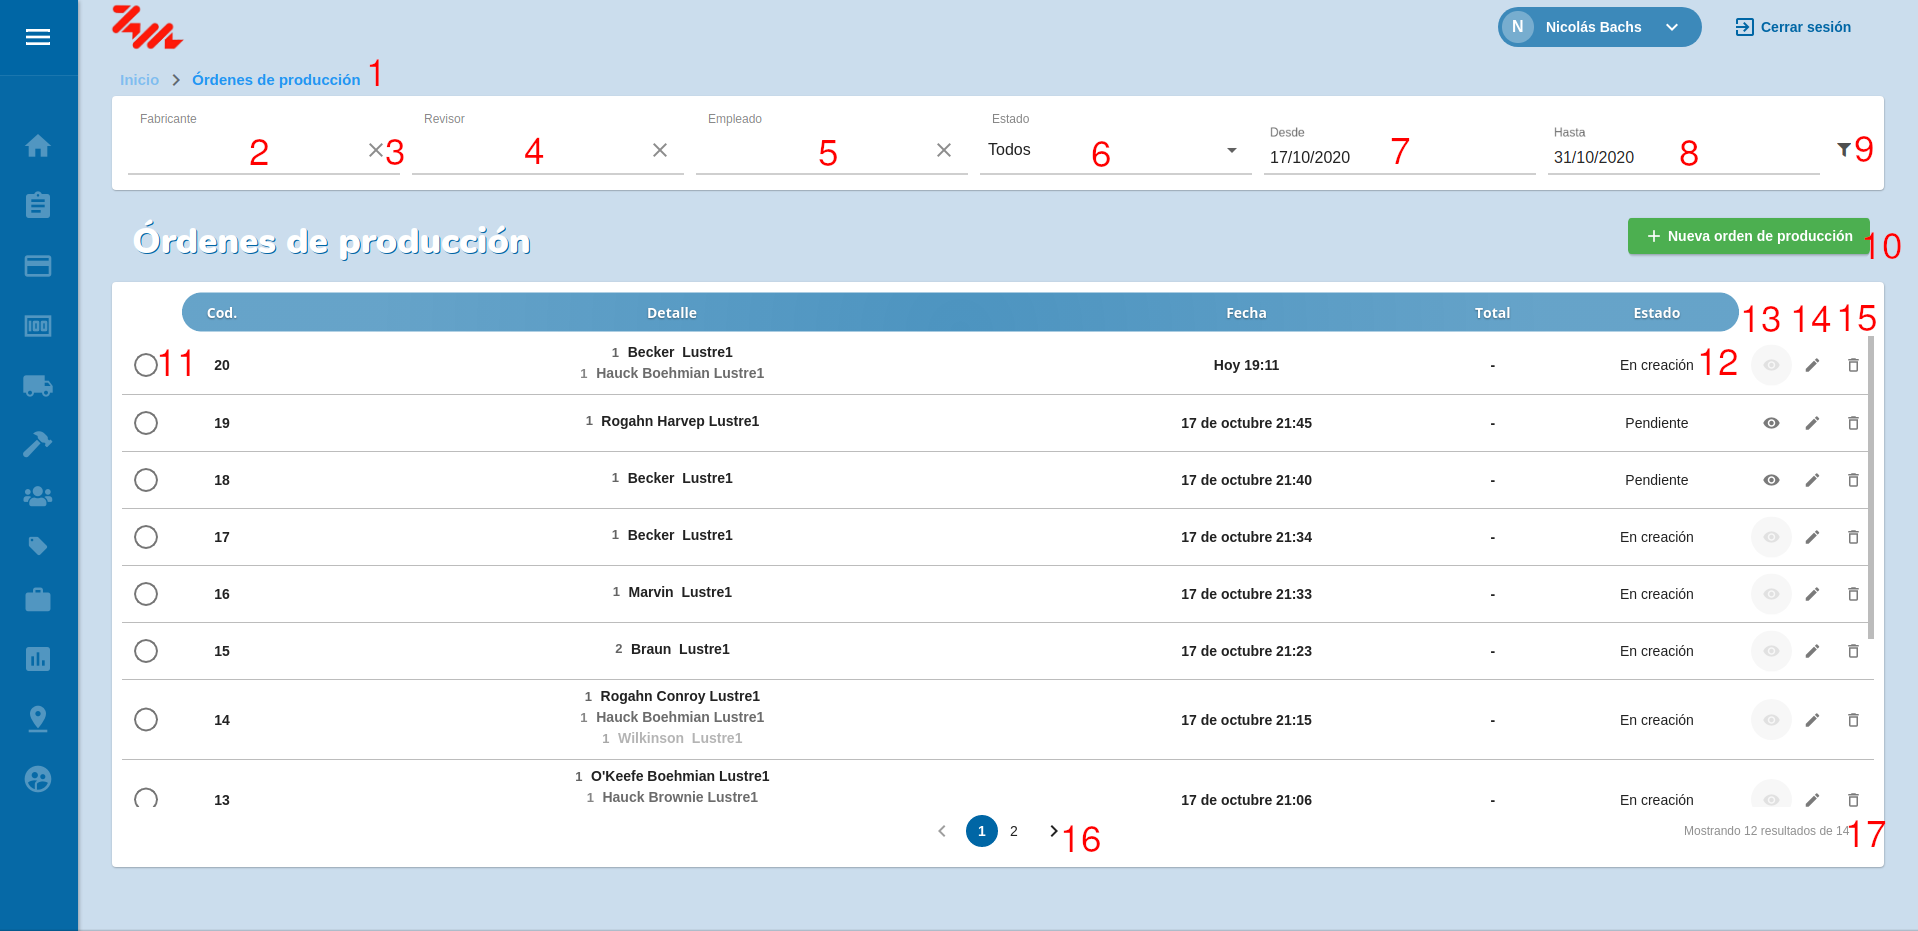
\includegraphics[width=\textwidth,height=\textheight,keepaspectratio]{Escenarios/AD-22-00}
\caption{Escenario - AD-22-00}
\label{fig:AD-22-00}
\end{figure}

Este escenario muestra toda la información referida a las órdenes de producción, junto con las acciones disponibles.
El botón \textbf{AD-32-01} permite navegar al escenario \textbf{AD-02-00}. El campo \textbf{AD-32-02} permite ingresar un fabricante para filtrar las órdenes de producción que tengan al menos una tarea designada a un determinado fabricante, el campo cuenta con el botón \textbf{AD-32-03} que permite borrar el texto ingresado en el campo. En el campo \textbf{AD-32-04} se puede indicar un empleado revisor para filtrar las órdenes de producción que hayan sido revisadas por un determinado empleado. Indicando un empleado en el campo \textbf{AD-32-05} se pueden filtrar todas las órdenes de producción que fueron creadas por un determinado empleado. La lista desplegable \textbf{AD-32-06} permite al usuario filtrar por los estados en los cuáles puede encontrarse la orden de producción. Los campos  \textbf{AD-32-07} y \textbf{AD-32-08} permiten al usuario filtrar las órdenes de producción de acuerdo a un rango de fechas en la cual fueron creadas. El botón \textbf{AD-32-09} permite visualizar más filtros de búsqueda disponibles, como ser el producto, la tela y el lustre, filtrando las órdenes de producción que contengan un detalle con alguno de éstos.
El botón \textbf{AD-32-10} permite al usuario crear una nueva orden de producción y navega al escenario \textbf{AD-23-00}.
El botón \textbf{AD-32-11} permite al usuario seleccionar una o más órdenes de producción del resultado de búsqueda. Si existen órdenes de producción seleccionadas se mostrarán botones con las opción de borrar las órdenes de producción seleccionadas. El campo \textbf{AD-32-12} muestra la información relacionada a las órdenes de producción especificando el código, el detalle de la orden de producción, la fecha de creación y el estado en el cual se encuentra. El botón \textbf{AD-32-13} permite navegar al escenario \textbf{AD-25-00} para ver la orden de producción, el botón \textbf{AD-32-14} permite al usuario editar la orden de producción navegando al escenario \textbf{AD-23-00} y el botón \textbf{AD-32-15} permite al usuario borrar la orden de producción. 
En \textbf{AD-32-16} se mostrarán las páginas de resultado, pudiendo cambiar de página. En \textbf{AD-32-17} se mostrará cuantos resultados se están visualizando y el total.
\clearpage
